\documentclass{neiuthesis} 
%\documentclass[draftthesis]{neiuthesis} 
\nocopyrightpage
\usepackage{amsmath}
\usepackage{natbib}
\usepackage[prependcaption,disable]{todonotes} %[obeyDraft]
\usepackage{Sweave}
% changes to Sweave.sty defaults
% from http://faculty.agecon.vt.edu/moeltner/AAEC5126/Sweave/docs/Arnholt_tutorial.pdf
\DefineVerbatimEnvironment{Sinput}{Verbatim}{fontsize=\small,fontshape=n}
\DefineVerbatimEnvironment{Soutput}{Verbatim}{fontsize=\small,fontshape=n}
\DefineVerbatimEnvironment{Scode}{Verbatim}{fontsize=\small,fontshape=n}
\usepackage{graphicx}
\usepackage{listings} 
\usepackage{courier} 
\lstset{breaklines=true,basicstyle=\ttfamily,language=R}
\usepackage{pdfpages}
\usepackage{pbox}
\usepackage{verbatim}
\usepackage{rotating}
\usepackage[normalem]{ulem}
\usepackage{hyperref}
\hypersetup{
  pdftitle={NEIU G\&ES MA Thesis},%
  pdfauthor={Neil Best <nbest@alum.mit.edu>},%
  pdfsubject={land use / land cover},%
  pdfkeywords={agriculture}{United States},%
  pdffitwindow=true,%
  pdfstartview={FitH}
}
\usepackage[all]{hypcap}
\usepackage{multirow}

\renewcommand{\topfraction}{0.85}
\renewcommand{\textfraction}{0.1}
\renewcommand{\floatpagefraction}{0.75}
% Be careful not to make \floatpagefraction larger than \topfraction, then you risk to produce a figure that can neither go on the top of a text page, nor on a page by itself.
% http://dcwww.camd.dtu.dk/~schiotz/comp/LatexTips/LatexTips.html#figplacement

\begin{document} 
\pagestyle{plain}
\bibliographystyle{chicago}

\title{Synthesis of a complete land use\slash land cover data set for
  the conterminous United States emphasizing accuracy in area and
  distribution of agricultural activity}
 

\othermasters{Master of Arts}{M.A.}  
\department{Geography \& Environmental Studies}

\author{Neil A. Best}
\degreeyear{August~2011}



\maketitle

%
\includepdf[pages={2,1}]{neiuForms.pdf}
%!pdfTeX error: pdflatex (file ./neiuForms.pdf): PDF inclusion: invalid font in reference type <dictionary>

\frontmatter

\begin{abstract} This paper presents an effort to produce a new land
  cover data set for the conterminous United States of America (cUSA)
  that augments available agricultural land use data with other uses
  and natural covers to create a complete landscape characterization.
  Using the Agland2000 data set as a benchmark we formulate a
  hybridization of the MODIS Land Cover Type (MLCT) for 2001 and the
  2001 National Land Cover Database (NLCD) that is particularly
  tailored to serve as an initialization data set for long-term
  economic land use change models.  In order to strike a balance
  between spatial precision and local diversity of use and cover the
  new data set has lower resolution than the MLCT ($5'$ vs. $15''$)
  but represents land use/land cover (LULC) components as sub-pixel
  fractions rather than discrete categories.  After aggregating to the
  $5'$ grid we present a method for decomposing the natural
  vegetation/cropland mosaic class found in MLCT into constituent
  classes as a function of the local landscape.  We then quantify its
  contribution to aggregate acreages by class, particularly cropland.
  We compensate for the absence of certain fine-grained details from
  MLCT, such as rural transportation networks, small settlements,
  linear water features, and wetlands, mainly due to sensor
  resolution, by incorporating corresponding components of the NLCD,
  after similar reclassification and aggregation, as a set of offsets
  to the MLCT-derived fractions.  The 175Crops2000 data set, valuable
  for its basis in per-crop agricultural production statistics, is
  used as a guide to further decompose the cropland areas into a set
  of crop-specific sub-categories designed to facilitate the economic
  modeling goals of the simulations that will be initialized by this
  data product.  The resulting data model is conceptually
  equivalent to a stack of spectral bands with the additional property
  that the components of each pixel sum to unity.  Its classification
  scheme is a mixture of a simplified version of the IGBP schema used
  in MLCT and a disaggregation of the monolithic cropland class that
  differentiates among the world's major commodity crops.  At each
  step of refinement we show that overall spatial distribution of
  cropland across the study area improves relative to the Aglands2000
  data set.  We close with a discussion of how this method might be
  applied globally and to successive years in the MLCT time series.
\end{abstract}


\chapter*{Acknowledgments}

\noindent This thesis is dedicated to my son, Leo.  Son, I began
working on this degree before you were born and my commitment to
completing it was sustained by my desire to demonstrate to you that in
life we finish what we have started.

\vspace{12pt}
\noindent I could not have completed this paper over the past year
and, by extension, my degree over more years than I care to mention,
without the support of my loving wife, Laura.

\vspace{12pt}
\noindent I want to thank Dr. Nicholas Kouchoukos of Lanworth,
Inc. for throwing me in the deep end of applying the open-source
geospatial software tool chain to spatial analysis of agriculture.

\vspace{12pt}
\noindent This work was made possible through the support of my
employer, the Computation Institute at the University of Chicago, and
its director, Dr. Ian Foster under the Community Integrated Model of
Economic and Resource Trajectories for Humankind project (CIM-EARTH,
\url{http://www.cim-earth.org/}) project.

\vspace{12pt}
\noindent My thesis committee was comprised of Dr. Monika Mihir
(chair), Dr. Erick Howenstine (department head), both of the
Department of Geography \& Environmental Studies at Northeastern
Illinois University, and Dr. Joshua Elliott from the Computation
Institute.  I deeply appreciate their guidance and support through all
stages of this project.


\tableofcontents 
\listoftables
\listoffigures

%% Create a List of Abbreviations. The left column %% is 1 inch wide and left-justified
\chapter{List of Abbreviations}

\begin{symbollist*}
\item[175Crops2000] Harvested Area and Yields of 175 crops (M3-Crops
  Data) \citep{Monfreda2008}
\item[Agland2000] Agricultural Lands in the Year 2000 (M3-Cropland and
  M3-Pasture Data) \citep{Ramankutty2008}
\item[AVHRR] Advanced Very High Resolution Radiometer
\item[CIM-EARTH] Community Integrated Model of Economic and Resource
  Trajectories for Humankind
\item[cUSA] conterminous (contiguous) Unites States of America, the ``lower 48''
\item[GADM] Global Administrative Areas, \url{http://www.gadm.org/}
\item[GIAM] Global Irrigated Areas Map
\item[GIS] Geographic Information Systems
\item[GMRCA] Global Map of Rainfed Crop Areas
\item[GLC2000] Global Land Cover 2000 \citep{EC2003}
\item[GRASS] Geographic Resources Analysis Support System, \url{http://grass.osgeo.org/}
\item[IGBP] International Geosphere-Biosphere Programme
\item[LULC] land use / land cover
\item[MODIS] Moderate Resolution Imaging Spectroradiometer
\item[MLCT] MODIS Land Cover Type \citep{MLCT}
\item[NLCD] National Land-Cover Database, 2001 \citep{Homer2004}
\item[PEEL] Partial Equilibrium Economic Land use model
\item[PLSS] Public Land Survey System
\item[RMSE] root of the mean squared error
\item[SPAM] Spatial Production Allocation Model
\item[SPOT] Syst\`eme pour l'Observation de la Terre

\end{symbollist*}

%% Create a List of Symbols. The left column 
%% is 0.7 inch wide and centered
\chapter{List of Symbols}

\begin{symbollist}[0.7in]
\item[$A_{min}$] Minimum sub-pixel fraction possible for primary cover
  given in MLCT base data
\item[$A_s$] Sub-pixel fraction of secondary cover type, function of
  classification confidence level and $A_{min}$
\item[$A_p$] Sub-pixel fraction of primary cover type, function of
  classification confidence level and $A_{min}$
\item[$\hat\theta$] Predicted sub-pixel fraction
\item[$\theta$] Observed sub-pixel fraction
\item[$'$] minute of arc, 1/60th of a degree
\item[$''$] second of arc, 1/60th of a minute, 1/3600th of a degree
\item[{[0,1]}] interval from 0 to 1, inclusive of 0 and 1; $0 \leq x \leq 1$ 
\item[[0,1)] interval from 0 to 1, inclusive of 0 but but not 1, $0 \leq x < 1$ 
%\item[$ \left[ 0,1 \right] $] interval from 0 to 1, inclusive of 0 and 1; $0 \leq x \leq 1$ 
%\item[$ \left[ 0,1 \right) $] interval from 0 to 1, inclusive of 0 but but not 1, $0 \leq x < 1$ 
\end{symbollist}


\mainmatter

\todototoc
\listoftodos


\chapter{Introduction}
\label{cha:introduction}

\section{Background}
\label{sec:background}

The continuing evolution and commoditization of high-performance
computing infrastructure is constantly opening new horizons in spatial
modeling of human\slash environment interactions.  Increases in
processing throughput, affordability of tera- and petabyte-scale
storage resources, and ubiquity of parallelization tools and
techniques create opportunities for formulating models of spatial
processes of increasing extent, granularity, dimensionality, and
complexity.  The intersection of geography, economics, and computer
science is a fertile frontier where researchers capable of harnessing
the utility of available technology are presented with an
unprecedented opportunity to contribute to resolving the urgent
questions of our time regarding humankind's outlooks for survival,
stewardship, and prosperity in coming decades and centuries.  These
issues generally revolve around characterizations of our manipulation
of natural processes, notably food production; the side effects of
those activities, being alterations of biogeochemical fluxes of matter
and energy within and into the biosphere \citep{Sellers1997}; and the
economic exchanges that mediate these activities as modulated by
policy.  Meaningful abstractions of these processes in the form of
iterative, process-based models that we can formulate in order to
derive descriptions of their dynamics and forecasts of their unfolding
are not possible without some detailed, spatially explicit
characterization of the ecological disposition of the earth's surface.
This ecology is to be inclusive of human ecology, which is to say
settlement, development, utilization, and transformation of natural
resources.  The general form of such a characterization is a land
use\slash land cover (LULC) map which depicts landscapes according to
categories of anthropogenic and natural phenomena \citep{Fisher2005a}.
\todo{Warning--page numbers missing in Fisher2005a} These maps are
necessarily functions of history, climate, geology, hydrology and are
formulated according to some design or convention with regard to their
constituent types and their definitions, which make possible myriad
representations of a given landscape regardless of scale.  When
conducting analysis in this space it is typically necessary to tailor
the analysis to accommodate available data or create new data from raw
physical measurements and observations, but a third option of fusing
aspects of multiple available data sets is also available, as we will
demonstrate here.

Arguably the most significant intersection of land use and land cover
is agriculture.  Agricultural activity has transformed all but the
most inhospitable, impervious, and inaccessible corners of the globe
and serves as a crucial underpinning of civilization, but is still an
expression of variability in weather, soils, and biology, natural
phenomena beyond humans' control, across the face of the earth.  In
the face of uncertainty regarding food security, availability of raw
materials for industry and trade, impacts and dynamics of
deforestation, desertification, and climate change, and sensitivity to
these alarming trends due to a burgeoning global population, reliable
forecasts of agricultural production and productivity over the long
term are objects of much desire in the corridors of government,
finance, and industry.

Recent years have seen a significant increase in the availability of
global land cover data sets including the University of Maryland
Global Land Cover Classification, Global Land Cover 2000 (GLC2000),
and MODIS Land Cover Type (MLCT).  At the regional level the National
Land-cover Database (NLCD) provides high-resolution LULC data for the United States and Puerto Rico.  These data sets are
summarized in Table \ref{tab:lulc} with pertinent references and
attributes of their collection.  The proliferation of these data sets
reflects the diversification and technological advances among
space-borne sensors in recent years, resulting in improved resolution,
both spatial and temporal, as well as innovation in post-processing
and classification algorithms that transform raw sensor data into the
thematic data that is readliy applicable to theoretical modeling.

\begin{table}[ht]
  \begin{center}
    \begin{small}
%\begin{sidewaystable}
      \begin{tabular}{p{1in}p{1in}p{0.5in}lp{0.5in}}
        \hline
        Data set & Reference & Sensor & Resolution & Time Span \\
        \hline
        UMD GLobal Land Cover 1998 & \citet{Hansen2000} & AVHRR & 1km & 1981 -- 1994 (composite) \\
        Global Land Cover 2000 & \citet{EC2003,Bartholome2005} & SPOT & 1km & Nov~1999~--~Dec 2000 (composite) \\
        National Landcover Database (NLCD) & \citet{Homer2004,Homer2007} & Landsat & 30 m & 2001 \\
        MODIS Land Cover Type v005 & \citet{MLCT,Friedl2010} & MODIS (Aqua~\&~Terra) & 500m & 2001~--~2008 (annual~time~series) \\
        \hline
      \end{tabular}
    \end{small}
    \caption{Summary of global LULC data sets}
    \label{tab:lulc}
  \end{center}
\end{table}
%\end{sidewaystable}

\todo{Check format of \autoref{tab:lulc}}

Similarly there has also been a proliferation of data sets that
describe the distribution and intensity of global agricultural
activity.  Some such as the Global Irrigated Areas Map (GIAM)
\citep{Thenkabail2008} and the Global Map of Rainfed Crop Areas
(GMRCA) \citep{Biradar2009} are the product of applying classification
techniques to large collections of remote sensing and GIS data.
Others such as Agricultural Land in the Year 2000 (Agland200)
\citep{Ramankutty2008}, Harvested Area and Yields of 175 Crops
(175Crops2000) \citep{Monfreda2008}, and the Spatial Production
Allocation Model (SPAM) \citep{You2006} are further informed by
agricultural production data published at national and sub-national
levels and disaggregated to grid cells within those boundaries
according to an optimization method described by \citet{YouWood2006}.
Data sets such as these have the potential to complement those of the
general comprehensive LULC category by offering additional information
on how to differentiate areas of cropland according to cultivars, and
farming practices such as crop rotation, multiple cropping, and
irrigation.


\section{Objective}
\label{sec:objective}

The Community Integrated Model of Economic and Resource Trajectories
for Humankind (CIM-EARTH) project at the University of Chicago's
Computation Institute, \url{http://www.cimearth.org/}, seeks to
provide a framework in which to combine the best of modern
computational and economic science to guide climate and energy policy.
A major facet of this work involves forecasting of land use change
over coming decades in the face of market pressures and hypothetical
climate change scenarios.  The supply side of this market analysis
depends, among other industries, on agriculture.  Prices of
agricultural commodities are sure to change in years ahead in response
to changes in technology, both of production itself and the products
and materials that are derived from them, changes in aggregate demand
for food and its attendant political ramifications, and changes to the
environments where agricultural production occurs.  Rents and prices
of land will follow from the profitability, adaptiblity, and risks
associated with the commodities that are possible to produce on it, as
well as costs of energy and inputs needed to bring those goods to
market.  A spatially explicit model of not only agricultural
production, but also the conversion of land into and out of active,
profitable cultivation is needed in order to make statements about the
magnitude, trend, volatility, and sustainability of agricultural
output to guide decisions about investment and policy.  We call this
the Partial Equilibrium Economic Land-use (PEEL) model, which refers
to the assumption of long-term demand trajectories as given inputs and
calculates the likely distribution of production needed to meet that
demand.  The foundation of this modeling effort would have to be a
LULC data set that is ``complete'' in the sense that it assigns all
land plus coastal and inland water areas to one category or another,
and that differentiates among crops to provide a modeling environment
where shifts in production factor allocation can be driven by market
and physical variables.  None of the data sets considered so far
exhibit these qualities; the LULC data sets treat cropland as a
homogenous category and the agricultural maps do not depict other uses
and covers.  Hence the motivation to develop a hybrid data set that
satisfies these criteria.

The mathematical properties of the PEEL model dictate a somewhat
unconventional data model for representing the allocation of land area
to the various LULC\slash crop categories.  Rather than assigning
individual grid cells to discrete categories as is typically done for
LULC maps, PEEL is formulated in a sub-pixel analysis framework, such
that for each cell a fraction is assigned to each category to
represent the degree to which that LULC type is present across the
area of the grid cell.  In a tabular representation the data would
show cells in rows and the LULC types in columns with a constraint
that the values in each row sum to unity.  In terms of geospatial
mapping this is equivalent to assigning a layer or band in a stacked
image set to each category, as is done for spectral bands in
radiometric data, and applying the same sum-to-one constraint to each
pixel.  \sout{An advantage to this approach is that errors of false
  spatial precision in higher-resolution data sets from which our
  inputs are derived, meaning that pixels in the mother data set are
  aggregated into an expression of probability across the larger model
  grid cell versus the definite location implied by the thematic data.
  It also means that we will have an avenue for increasing model
  complexity and the raw size of the data set by a linear factor by
  increasing the depth of the data array rather than the quadratic
  increase that accompanies increases in resolution.} \todo{Does
  everyone agree that we can do without this passage?}  The primary
purpose of this design choice is to strike a balance between
locational specificity and a convenient accounting mechanism for land
use conversion forecasts that would only confer false precision and
impose additional computational burden if expressed spatially.  In
other words, the land area of a pixel is considered to be a single
location whose internal arrangement is unspecified.  The model can
incorporate constraints governing the iterative transition of those
fractions that are stated algebraically in order to exclude protected
natural areas from conversion or require a degree of autocorrelation
among neighbors to prevent unrealistic divergences in development
patterns among grid cell neighborhoods, for example.

A disadvantage of this data model is apparent when attempting to
visualize the data.  A thematic map can be viewed in a single pass
given a well-designed palette that has a reasonable number of classes
and the relative proportions and distributions of classes can be
readily perceived by the viewer.  For the sub-pixel data model a
cognitive adjustment is necessary in order to consider multiple
classes simultaneously.  Although it is possible to employ the
false-color approach typically used for viewing multispectral data,
which is to map a subset of three bands to the red, green, and blue
channels, this limits a given map to portraying three classes
simultaneously, or else picking two of primary interest and lumping
the remaining fractions into a catch-all category.  This method is not
quite as applicable to categorical data that we are discussing as it
is to spectral data because a set of three spectral bands are
typically left in long-to-short wavelength order and reassigned to
red, green, and blue, which amounts to shifting their frequencies into
the visible spectrum, in order to produce a false-color image.  It
would be difficult to interpret the mixing of thematic hues or the
arbitrary assignment of categories to primary hues.  The approach to
visualization taken for this paper is to render maps in individual
layers with a uniform palette to express the fractional expression of
the classes and distinguish zero from null outside the set of pixels
included by the analysis mask.  Interpretation is aided by presenting
these maps in collections called facets in Wilkinson's
\citeyearpar{Wilkinson2005} grammar of graphics to convey the full
depth of information in consideration.

Given that the CIM-EARTH modeling framework is in a prototype phase we
are taking a conservative posture towards the degree of detail that we
wish to capture in early applications.  This is expressed by the
choice of resolution of our model grid and the number of LULC
categories, including crop sub-categories, to which each cell can be
allocated.  With an ultimate goal of running simulations at global
extents we wanted to err on the side of prudence before measuring the
computational requirements of processing time and storage of a working
prototype.  Early tests gauging the computational requirements for
carrying out these simulations have indicated that operating on a 5$'$
grid cell globally is not prohibitively costly in time, memory, or
storage and that the design, implement, evaluate iterative development
cycle can proceed at a satisfactory pace.  This choice of resolution
is not as arbitrary as it may seem given that it equates to roughly
10km at the equator and happens to be the same resolution as some of
the base data employed in this exercise.

The algorithm described here will be peformed on the subset of the
global 5-arc-minute grid that contain land area of the 48 contiguous
states of the United States but is intended to be applied globally.
As we will discuss in Chapter \ref{cha:datasets} when the base data
sets are described in greater detail the MLCT is chosen as the
foundation of this method because of its global coverage and greatest
resolution among global data products.  As the technique presented in
Chapter \ref{cha:analysis} matures it will be applied globally and
also extended in time to convert the proceeding years of the MLCT time
series to a form useful in the PEEL model.  This will be important for
model validation to show that the model is capable of producing an
evolution of the overall state of land use that corresponds to
available observations.  As we will see the necessary information
needed to obtain a realistic distribution of areas for all classes is
not currently available.  We use the NLCD to complement MLCT for
certain classes that are too small to resolve at 500m, hence the
restricted extent for which this method is currently feasible.  In
Chapter \ref{cha:conclusions} we wrap up with a discussion of the
merits of this endeavor and propose future avenues of research based
thereon.

At this time we are not aware of any other systematic attempt to
incorporate the full depth of information offered by MLCT, which is a
collection of three map layers: a primary cover class, a confidence
level for that primary classification, and a secondary classification.
Rather than interpret the secondary classification as the next most
likely possibility we accept this triplet as an expression of the
sub-pixel composition of that area.  Aggregation of MLCT from 15
$''$ to 5$''$ will blur the spatial precision implied
by this formula and treat the local $20 \times 20 \times 3$ array as a
probabilistic expression of the local landscape composition.  We will
show that this approach, given a principled assumption about the
relationship between confidence level and sub-pixel area, that
aggregate acreage estimates of the LULC classes, particularly
cropland, are improved through this method.  More on this in Section~\ref{sec:mlct}.

\section{Reproducible Research}
\label{sec:reproducible}

We maintain that the manner in which we execute this analysis is as
significant, if not more so, to the practice of geospatial analysis as
the product of the analysis itself.  The second objective of this
paper is to demonstrate the concept of reproducible resarch in
geospatial analysis that has been made possible by a suite of
open-source software tools.  Previous to employing the suite of tools
described below, our typical research experience with widely available
GIS software, both free and commerical, is to conduct the analysis in
a graphical user interface (GUI) environment and capture outputs for
publication by manually exporting maps and charts as images and
transcribing quantitative results from on-screen displays into the
body of a document.  Whenever an adjustment is made the maps, charts,
tables, and quantities in the paper must be updated manually.  The
open-source GIS software package
\href{http://grass.osgeo.org/}{\texttt{GRASS}} \citep{GRASS} employs a
command-line oriented interface as its basic mode of user interaction
which makes recording of steps in an analysis in the form of a script
a more approachable undertaking once the user develops familiarity
with the necessary commands, but due to \texttt{GRASS}'s decades-long Unix
heritage, this scripting is done using the Bash shell, a system that
was designed primarily for system administration and suffers from a
byzantine syntax and a dearth of native data structures, making
succinct, expressive programming difficult.

The \href{http://www.r-project.org/}{\texttt{R}} statistical package
addresses these shortcomings \citep{R} by virtue of its design's
orientation towards mathematical and statistical analysis.  Using
Robert Hijmans' \citeyearpar{Hijmans2011} \texttt{raster} package for
\texttt{R} provides an interface for accessing and analyzing
geospatial raster data sets without being forced to load the entire
data set into memory, a constraint that has historically been the case
with \texttt{R} data in general and made operations on large
geospatial data sets difficult.  Friedrich Leisch's
\citeyearpar{Leisch2002} \texttt{Sweave} package for \texttt{R} is a
tool for embedding \texttt{R} code within a
\href{http://www.latex-project.org/}{\LaTeX} \citep{Lamport1994}
document for inline code evaluation and dynamic injection of figures,
tables, and text into a document prior to final typesetting.  The
utilization of these tools results in a software environment where the
princples of reproducible research described and demonstrated by
\citet{Gentleman2007} can be applied.  An academic paper produced
under this paradigm is analogous to a piece of open-source software
where the majority of ``users'' will simply want the ``compiled''
version in the form of a PDF document, but the author also provides
access to the the source code behind the production of that document
for inspection, re-execution, and adaptation for follow-on research.
This approach lowers the costs of reproduction and verification of
scientific analyses, central tenets of the scientific method that have
effectively fallen out of practice due to these costs.  With the
advent of software tools such as these this approach to documenting
research has gained a foothold in numerous desciplines from statistics
to medical imaging.

The tables, charts, and maps included in this document are generated
by \texttt{R} code which will be included as an appendix.  The maps
and charts are produced using Hadley Wickham's
\citeyearpar{Wickham2009} \texttt{ggplot2} package, employing the
grammar of graphics mentioned above.  David Dahl's \texttt{xtables}
package is used to convert \texttt{R} data frames into tables
marked-up for typesetting.  \texttt{Sweave} itself provides a facility
for injecting the results of evaluating arbitrary \texttt{R}
expressions in the text body, making it possible to render pieces of
data, such as total acreages, in a dynamic fashion within the body of the text.

The source code of this paper will be submitted on optical media to
Northeastern Illinois University's Graduate college along with the
final draft.  It will also be available via GitHub at
\url{https://github.com/nbest937/thesis}.  The initial, intermediate,
and final data products will be made available for download either
through \url{http://www.ci.uchicago.edu/~nbest} and\slash or
\url{http://www.cimearth.org/} by request to
\url{mailto:nbest@ci.uchicago.edu} or \url{mailto:nbest@alum.mit.edu}.

s% -*- mode: noweb; noweb-default-code-mode: R-mode; -*-








\graphicspath{ {datasets/} }


\chapter{Data Sets}
\label{cha:datasets}

This chapter presents summary descriptions of the various data sets
that are relevant to this analysis and further discussion on how they
were manipulated in preparation for analysis.  Operations where
multiple data sets are used in conjunction are deferred to Chapter
\ref{cha:analysis}.

The general approach with the MLCT and NLCD data sets is to reclassify
their categories, calculate per-pixel, per-class areas at the native
resolutions, and aggregate the new classification to the 5$'$ grid.
The purpose of the reclassification is to reduce the number of classes
and have a uniform set of classes across data sets.  The challenge in
this is that classification defintions are sometimes subtly different
which makes direct comparison across data sets somewhat subjective, so
we describe the mapping between original and simplified
classifications.  We apply and aggregation operation that calculates
the relative proportion of each class in the new classification system
present in each 5$'$ grid cell according to the base data.  In this
process we convert classified maps whose pixels have discrete values
to a stack of maps, one map per class, whose pixels have real number
values on the interval $[0,1]$ representing fractional areas and are
constrained to sum to unity for each pixel through the stack.  In the
general case of the MLCT data product the process converts two
discrete, thematic variables and one continuous variable, those being
a primary covery type, a secondary cover type, and classification
confidence level respectively, into a set of continuous variables
representing fractional areas for the cover types in the siplified
classification system.  This general case is also compared to simpler
cases of the NLCD and considering only the primary classification of
MLCT.  In these cases the process is simplified by considering only a
primary thematic layer and performing the aggregation without a
secondary cover type or confidence level by which to relate them but
we are able to reuse the same functions for the raster calculations.

To illustrate the process of converting the these data sets from their
original representation we are including maps of an area of
southeastern Michigan to show greater detail through each step of the
process.  We chose this region for its diversity of land covers and
uses, its relative diveristy of agricultural commodities across its
significant cropland area, the significant presence of the mosaic
class to illustrate our method for its decomposition and its
familiarity to our principal author, being his brthplace.


\section{MODIS Land Cover Type (MLCT)}
\label{sec:mlct}

In preparation for this analysis we prepared the 2001 MLCT data by
patching together the tiles as delivered in the equal-area sinusoidal
projection, reprojecting that mosaic to geographic coordinates, and
extracting a subset for the conterminous United States (cUSA).  These
preparation steps were carried out in a \texttt{GRASS} database prior
to the adoption of the reproducible research framework for this paper,
so those steps are not demonstrated here.  The cUSA study area is
defined as the set of 5$'$ grid cells that intersect with the cUSA
polygon in version 1 of the Global Administrative Areas (GADM) vector
data set, which includes the water bodies on the American side of the
international border across the Great Lakes, but does not extend to
oceanic waters beyond the coastal grid cells that intersect with any
land mass.

In this section we will demonstrate the process of converting the MLCT
data from its native form, consisting of primary cover type,
classification confidence for the primary cover, and secondary
(alternate) cover type at 15$''$ resolution, to a stack of cover
fractions at 5$'$ resolution using the simplified cover/use
classification specified by the PEEL model.

\subsection{Reclassification}
\label{sec:mlct-reclass}

The following table shows the mapping of the IGBP classes used in the
original MLCT data to the simplified classification designed for the
PEEL model.

\missingfigure{MLCT reclassification table}





\begin{figure}[hpt] 
  \centering
  

\includegraphics{fig_thumb_pri_reclass}
%\end{center} 
\caption{MLCT primary cover reclassified detail} 
\label{fig:thumb_pri_reclass} 
\end{figure} 

\todo{Is this figure any better placed than others?}

\autoref{fig:thumb_pri_reclass} shows the result of reclassifying the MLCT data
for our detailed study area.  From this map we see that this area is
dominated by the crop class in the north and the mosaic class to the
south with scattered forests and pockets of development throughout.
The urban complex of Port Huron, Michicagn and Sarnia, Ontario is
visible in the southeast corner.  along with the confidence level given for
the primay classification.

\begin{figure}[hpt] 
\begin{center}
  

\includegraphics{fig_thumb_sec_reclass}
\end{center} 
\caption{MLCT secondary cover reclassified detail} 
\label{fig:thumb_sec_reclass} 
\end{figure} 


In \autoref{fig:thumb_sec_reclass} we notice that areas in the
northern and central sections of the map that were classified as crop
in the primary layer have null values in the secondary class.  It is
apparent that where a secondary class is given that the mosaic class
is often indicated where the primary class indicates cropland and vice
versa.  It is possible for primary and secondary classes to be
assigned to the same category because of the reclassification step.
When one of our pixels indiactes the forest class for both its primary
and secondary classifications it simply reflects a distinction between
sub-types of forest in the original data, for example evergreen and
deciduous.

\begin{figure}[hpt] 
\begin{center}
  

\includegraphics{fig_thumb_pct}
\end{center} 
\caption{MLCT primary cover classification confidence} 
\label{fig:thumb_pct} 
\end{figure} 

\autoref{fig:thumb_pct} shows the confidence level as a percentage.
We see that the areas where no secondary class is given are areas
where confidence is 100\% and the primary classification is cropland
and therefore would be accounted as 100\% cropland by area by any
method of adding up these areas.  In light of this observation it is
clear that MLCT will generally over-estimate cropland because it is
certain that these areas are not completely under cultivation but
rather are interspersed with homesteads, fence lines, small wood lots,
roads, and such cultural features.  In areas such as this that were
made available for settlement in the 19th century according to the
Public Land Survey System (PLSS) we expect to find roads delineating
every square mile in general.  

The relationships described among the three layers of the MLCT are
perhaps more easily appreciated visually by mapping the individual
classes separately.  \autoref{fig:thumb_pri_facet} does this for the
primary class in our example detail area and
\autoref{fig:thumb_sec_facet} for the secondary class.


\begin{figure}[hpt] 
\begin{center}
  

\includegraphics{fig_thumb_pri_facet}
\end{center} 
\caption{MLCT primary covers shown separately, detail} 
\label{fig:thumb_pri_facet} 
\end{figure} 


\begin{figure}[hpt] 
\begin{center}
  

\includegraphics{fig_thumb_sec_facet}
\end{center} 
\caption{MLCT secondary covers shown separately, detail} 
\label{fig:thumb_sec_facet} 
\end{figure} 

%\subsubsection{Analysis Area}
%\label{sec:reclass-analysis-area}

Conveniently we are able to reuse the same functions for
reclassification and mapping of the data that we have prepared for the
larger study area.  \autoref{fig:mlct_pri_reclass} shows the map of
the primary classification across the cUSA, and likewise
\autoref{fig:mlct_sec_reclass} for the secondary layer and
\autoref{fig:mlct_pct} for the confidence level.  Because the maps are
showing a greater extent in relatively the same amount of page space
it is even more useful to create the facet maps for the individual
classes as \autoref{fig:mlct_pri_facet} and
\autoref{fig:mlct_sec_facet} have done.  From these maps familiar
generalities of the cUSA's geography are more apparent, such as the
prevalence of forests in the east and northwest, cropland in the
midwest, shrub lands in the southwest and open lands across the west.
It is interesting to note that the mosaic class is primarily
concentrated in the eastern portion of the study area which we can
attribute to greater population density, topography, and historical
patterns of settlement resulting in characteristically smaller parcels
and a greater degree of mixing among agricultural uses and natural
covers.



\begin{figure}[hpt] 
\begin{center}


\includegraphics{fig_mlct_pri_reclass_trim}
\end{center} 
\caption{MLCT primary cover reclassified} 
\label{fig:mlct_pri_reclass} 
\end{figure} 


\begin{figure}[hpt] 
\begin{center}
  

\includegraphics{fig_mlct_sec_reclass_trim}
\end{center} 
\caption{MLCT secondary cover reclassified} 
\label{fig:mlct_sec_reclass} 
\end{figure} 


\begin{figure}[hpt] 
\begin{center}
  

\includegraphics{fig_mlct_pct_trim}
\end{center} 
\caption{MLCT primary cover classification confidence} 
\label{fig:mlct_pct} 
\end{figure} 


\begin{figure}[hpt] 
\begin{center}
  

\includegraphics{fig_mlct_pri_facet}
\end{center} 
\caption{MLCT primary covers shown separately} 
\label{fig:mlct_pri_facet} 
\end{figure} 


\begin{figure}[hpt] 
\begin{center}
  

\includegraphics{fig_mlct_sec_facet}
\end{center} 
\caption{MLCT secondary covers shown separately} 
\label{fig:mlct_sec_facet} 
\end{figure} 


\subsection{Aggregation}
\label{sec:mlct-aggr}

MLCT has a nominal resolution of 500m which roughly equates to 15$''$
at the eqautor and so is conveniently an even division of the 5$'$
grid to which we wish to aggregate it, the two related by a factor of
20.  Therefore each cell in the output of this aggregation will be a
function of the 400 orginal MLCT pixels within its footprint.  The
dataset consists of a primary classification, along with a measure of
confidence up to 100\%, and a secondary classification.  The secondary
cover type is given as the most likely alternative to the primary type
\citep{Friedl2010}, but for purposes of our analysis we are taking a
more probabilistic view and incorporating all available information
from the base data.  Because we are aggregating the data up to
5-arcmin resolution there is no expectation that the sub-pixel
fractions at full resolution are spaitally specific, but in the
aggregate our characterization of each grid cell's composition will be
nuanced by this additional information.  The primary class covers at
least roughly 50-60\% of a given pixel $x$, and this percent is almost
certainly a monotonically increasing function of the confidence
measure $c$.  \todo{cite email from Friedl}.  For the purposes of this
analysis we assume that this dependence is linear. Thus, for the
primary and secondary cover types in a pixel:

$$
A_p(x) = A_{min} + (1 - A_{min}) c(x)
$$
$$
A_s(x) = 1 - A_p(x)
$$

where $0.50 \le A_{min} \le 0.60$ is primarily chosen based on an
interpretation of $c$.  Given that there are only a handful of
examples of $c < 0.20$ \todo{consider including histograms showing
  confidence distribution}, setting $A_{min} = 0.50$ is appropriate.
Certainly for a classification to be considered the primary it must
represent a bare majority of the area covered by that pixel at
minimum, and the distributions of confidences indicate that the vast
majority of pixels contain greater than 60\% of their area in the
primary under the rubric described above.  The equations are simplified
as follows by assuming this value for $A_{min}$.

$$
A_p(x) = \dfrac{1 + c}{2}
$$
$$
A_s(x) = 1 - A_p(x) = \dfrac{1-c}{2}
$$

% will this help?



Applying these formulae results in a map for each cover type where the
pixel values are the sub-pixel areas on the interval $[0,1]$.  The map
of the fraction of the primary cover type is visually equivalent to
that of the classification confidence level because the former is
simply a linear scaling and offset of the latter.  \autoref{fig:thumb_fracs} shows the result of calculating $A_p + A_s$ for each individual class.  

%\subsubsection{Detail Area}
%\label{sec:agg-detail-area}


\begin{figure}[hpt] 
\begin{center}
  

\includegraphics{fig_thumb_fracs}
\end{center} 
\caption{Sub-pixel fractions at original resolution for $A_{min}=0.5$}
\label{fig:thumb_fracs}
\end{figure} 

By way of comparison we also consider the trivial case of settimg
$A_{min} = 1$ which indicates that the secondary cover is ignored
altogether and the primary cover is taken to represent 100\% of the
pixel area.  \autoref{fig:thumb1_fracs} shows these difference.  The
effect of adjusting $A_{min}$ is subtle; we will examine it more
closely after aggregating to the 5$'$ grid.

\begin{figure}[hpt] 
\begin{center}
  

\includegraphics{fig_thumb1_fracs}
\end{center} 
\caption{Sub-pixel fractions at original resolution for $A_{min}=1$}
\label{fig:thumb1_fracs}
\end{figure} 

Computationally the process of converting the reclassified maps to
sub-pixel fractions at the desired 5-arcmin resolution is a three-step
process.  First we calculate the fraction of the primary cover type as
a function of the classification confidence as described above.  Next,
a sub-pixel fraction for each cover type is calculated at full
resolution, recognizing that the primary and secondary classes may be
identical after the reclassification, such as cases where the original
data indicated two different type of forests.  Aggregating to a
coarser resolution is a simple matter of calculating the mean of these
values over the intersecting pixels at the original resoution.
Because the desired 5$'$ resolution is a multiple of the original
15$''$ resolution the pixels are perfectly nested, which is
convenient for properly computing this mean.


\begin{figure}[hpt] 
\begin{center}
  

\includegraphics{fig_thumb_agg}
\end{center} 
\caption{Aggregated sub-pixel fractions for $A_{min}=0.5$}
\label{fig:thumb_agg}
\end{figure} 

\begin{figure}[hpt] 
\begin{center}
  

\includegraphics{fig_thumb1_agg}
\end{center} 
\caption{Aggregated sub-pixel fractions for $A_{min}=1$}
\label{fig:thumb1_agg}
\end{figure} 


Before proceeding further it is interesting to inspect the differences
between the aggregated maps for the chosen values of $A_{min}$ as
shown in \autoref{fig:thumb_agg_diff}.  Positive values indicate that
$A_{min} = 0.5$ resulted in a greater fraction.  The main message from
this chart is that considering the secondary cover class results in
greater mixture between the crop and mosaic classes because cropland
is reduced in the north of the detail area where it was dominant in
the primary land cover type, and simlarly for mosaic in the south.
The relative suitability of these choices for $A_{min}$ is discussed
in \autoref{cha:analysis}.



\autoref{fig:thumb_agg_diff} emphasizes the difference between the
choice of $A_{min}=0.5$ and $A_{min}=1.0$ for the calculation of the
sub-pixel fractions and their aggregation to 5$'$ with a difference
map.  Positive values in the map indicate areas where $A_{min}=0.5$
produced a greater value.  We see more clearly from this set of maps
that the effect of considering the secondary class results in a shift
of up to 10\% of total cell area from crop to mosaic in the north of
our detail area and vice versa for the southern portion.  This
decrease in the relative dominance of the primary class is expected as
we saw from the earlier maps (\autoref{fig:thumb_pri_facet} and
\autoref{fig:thumb_sec_reclass}) of the MLCT data which classes were
indicated by the secondary classes in those areas.

\begin{figure}[hpt]
\begin{center}
  
%def

\includegraphics{fig_thumb_agg_diff}
\end{center} 
\caption{ Difference of aggregated sub-pixel fractions}
\label{fig:thumb_agg_diff}
\end{figure} 

%\subsubsection{Analysis Area}
%\label{sec:agg-analysis-area}


We apply the same functions for calculating the 15$''$-resolution map
of the primary cover class as a function of the confidence level $c$
for the entire cUSA study area, converting those to per-class
fractions at the same extent and scale, and aggregating those values
to the 5$'$ grid.  The corresponding figures are not shown because the
decrease in relative resolution makes interpretation difficult.  Based
on the behavior that these functions exhibited over the detail area we
can be confident that they will perform correctly over the greater
extent.



\subsection{Mosaic decomposition}
\label{sec:decomposition}

The MLCT classification includes a type that is problematic for the
economic models for which this data set is intended, the ``cropland /
natural vegetation mosaic'' class.  This class is defined as a hybrid
of cropland and some mixture of natural covers (forest, shrub, or
open) with no single component exceeding 60\% \citep{Friedl2002} and
croplands generally comprising 40--60\% of pixel area \todo{cite Friedl
  email}. Being a hybrid of developed land use and natural land cover
we wish to differentiate the cropland from the natural vegetation in
order to calculate a more meaningful total for cropland area and
thereby eliminate the mosaic class from the final tabulation.  In the
present implementation of the reclassification and aggregation process
we are making three very simple assumptions about the composition of
area delineated as mosaic lands:

\begin{enumerate}
\item Mosaic land is 50\% cropland.
\item The other 50\% is a blend of forest, open, and shrub in
  proportion to the expression of those classes in the same 5-minute
  cell.
\item In the absence of such information we simply assume that the
  natural component of the mosaic is an equal blend of all three.
\end{enumerate}

The intention here is to make simplifying assumptions that will allow
us to proceed with the evaluation of this analytical framework.
Although it may be interesting to vary the proportion used to
calculate the proportion of mosaic land to be allocated to crop land
we have no principled basis for this as of yet, considering that the
defintion implies that this proportion is variable across the MLCT
rather than being some unknown single-valued quantity.  The choice of
the 50\% level reflects the assertion that the mosaic is a cultural
class grouped with cropland and urban in the IGBP classification
scheme without overstating the degree of development.  MLCT provides
adequate variability in this dimension by commonly pairing cropland
and mosaic in the primary/secondary class data.  The second assumption
imposes that 15$''$ mosaic cells' non-crop portion will have the same
relative composition of forest, open, and shrub as the as the
non-mosaic portion of the 5$'$ grid cell in which it falls. Therefore
mosaic pixels in a 5$'$ cell where only forest is found of the three
non-crop mosaic components will be allocated 50\% crop and 50\%
forest.  \autoref{fig:thumb_nomos} and \autoref{fig:thumb1_nomos} show
the effect of decomposing the mosaic class in this fashion for
$A_{min}$ values of 0.5 and 1.0 respectively.



\begin{figure}[hpt]
\begin{center}
  


\includegraphics{fig_thumb_nomos}
\end{center} 
\caption{Aggregated cover fractions after mosaic decomposition, $A_{min}=0.5$}
\label{fig:thumb_nomos}
\end{figure} 

\begin{figure}[hpt]
\begin{center}
  


\includegraphics{fig_thumb1_nomos}
\end{center} 
\caption{Aggregated cover fractions after mosaic decomposition, $A_{min}=1.0$}
\label{fig:thumb1_nomos}
\end{figure} 



\begin{figure}[hpt]
\begin{center}
  

\includegraphics{fig_thumb_nomos_diff}
\end{center} 
\caption{Differences of sub-pixel fractions after mosaic
  decomposition, positive when $f(A_{min} = 0.5)$ is greater}
\label{fig:thumb_nomos_diff}
\end{figure} 





Our hypothesis from the outset is that there is information worth
capturing in the secondary class and classification confidence level
provided by MLCT.  We will test this hypothesis in
\autoref{cha:analysis} but in order to do so we need an ``observed
truth'' to provide an independent standard by which to make a
comparison on the basis of overall reduction in error at the 5$'$ grid
cell level.  The following section describes such a data set which
will be held up against these MLCT-derived data sets in the next
chapter.

% more appropriately addressed in following chapter

% Both 5-arcmin data sets derived from the MLCT in this fashion
% overestimate cropland area relative to that indicated by Agland2000,
% but the $A_{min} = 0.5$ variant better portrays the spatial variation
% judging from a simple root-mean-squared-error (RMSE)
% test. \todo{illustrate/demonstrate the RMSE test on the 5-arcmin MLCT
%   data sets}

\section{Agricultural Lands in the Year 2000 (Agland2000)}
\label{sec:agland2000}


The data set described by \citet{Ramankutty2008}, referred to in this
paper as ``Agland2000'', is the product of an effort to merge
satellite-derived LULC classifications with census data of
agricultural actviity compiled at national or sub-national levels
according to availability on around the turn of the last century.  It
uses both an older version of the MLCT (known as BU-MODIS) and the
GLC2000 data set mentioned in \autoref{sec:background} and a mask
based on climatic criteria and delineations of protected areas to
allocate the census data to the 5$'$ grid for both cropland and
pasture.  The ``open'' class in this data set has been renamed from
``pasture'' in its creator's nomenclature, but it is clear from its
ditribution shown in \autoref{fig:agland} that it represents a
phenomena that is not apparent in the MLCT data, so we do not attempt
to use it or reconcile it here, rather only carry it along to a small
degree for sake of comparison.  We attribute this discrepancy to
commingling of managed pasture lands and natural open land in the MLCT
classification.  It is important to note that Agland2000 is used as an
input into the classification algorithm of the version of MLCT that we
are using here and acknowledge the possibility of circularity when
comparing the two, but because of its basis in census data we will use
the cropland component of Agland2000 as an ``observed truth'' for the
purposes of evaluating our incremental adjustments to the maps we
derive from MLCT in \autoref{cha:analysis}.
  
%def 

\begin{figure}[hpt]
\begin{center}
  

\includegraphics{fig_thumb_agland}
\end{center} 
\caption{Agland2000 distribution in detail area}
\label{fig:thumb_agland} 
\end{figure} 

\begin{figure}[hpt]
\begin{center}
  

\includegraphics{fig_agland_trim}
\end{center} 
\caption{Agland2000 distribution in cUSA study area}
\label{fig:agland} 
\end{figure} 


\begin{comment}
\section{Major Land Uses (MLU)}
\label{sec:mlu}

This is a tabular data set published by the Economic Research Service
(ERS) at the USDA of land acreages by various uses and covers at a
state level.  We hope to compare our results to this data on a
state-by-state basis in order as a check and possibly incorporate some
of its information as a refinement.

\end{comment}

\section{National Land-cover Database 2001 (NLCD)}
\label{sec:nlcd}

\citet{Homer2004}


The NLCD gives a higer-resolution (30m) snapshot of LULC circa 2001.
\todo{check whether/how urban, water, wetland are informed with priors
  in NLCD} Reclassifying and aggregating this data to 5-arcmin
resolution in a fashion similar to that used for the MLCT is expected
to give better estimations of aggregate area for detailed features
like rural transportation networks and small stream and wetland
features.  This will compensate for MLCT's bias against these finely
detailed structures due to it's resolution.  It is the availability of
this information that makes it difficult to apply this analysis beyond
the United States without access to a comparable data set with global
extents.  The analysis is restricted to the conterminous US because of
the relative paucity of agricultural activity in Hawaii and Alaska.

As with the MLCT the process of reclassification and aggregation is
performed for both the detail region and the complete region.

One limitation of the \texttt{raster} library for \texttt{R} that we
are using is that the aggregation function requires that the output
resolution be a multiple of the output resolution.  The 30m resolution
of the NLCD equates to 1.25361$''$ and so does not satisfy this
requirement.  This deficiency was addressed by resampling the input to
1.25$''$ resolution prior to export from \texttt{GRASS} for this
analysis using a nearest-neighbor sampling algorithm, which gives an
even factor of 240 between the two resolutions.

\todo{Incorporate Joshua's suggestion to show further NLCD detail to better illustrate the discrepancy in developed areas}


\subsection{Reclassification}
\label{sec:nlcd-reclass}

\missingfigure{NLCD reclassification table}


\begin{figure}[hpt] 
\begin{center}


\includegraphics{fig_thumb_nlcd_reclass}
\end{center} 
\caption{NLCD reclassified} 
\label{fig:thumb_nlcd_reclass} 
\end{figure} 

\begin{figure}[hpt] 
\begin{center}
  

\includegraphics{fig_thumb_nlcd_facet}
\end{center} 
\caption{NLCD covers shown separately, detail} 
\label{fig:thumb_nlcd_facet} 
\end{figure} 

\subsection{Aggregation}
\label{sec:nlcd-aggr}

The same code used for refactoring the MLCT when considering only the
primary cover type can be applied here.

Repeating this process for the entire study area is computationally
expensive due to the NLCD's high resolution.


 

\begin{figure}[hpt] 
\begin{center}
  


\includegraphics{fig_thumb_nlcd_agg}
\end{center} 
\caption{NLCD aggregated cover fractions, detail area}
\label{fig:thumb_nlcd_agg}
\end{figure} 




\begin{figure}[hpt] 
\begin{center}
  


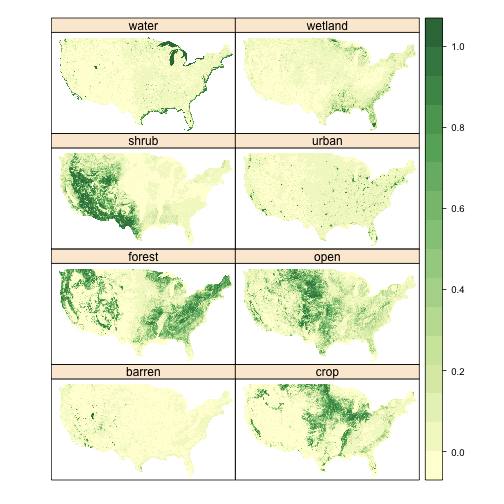
\includegraphics{fig_nlcd}
\end{center} 
\caption{NLCD aggregated cover fractions}
\label{fig:nlcd}
\end{figure} 

\begin{comment}
\section{Cropland Data Layer (CDL)}
\label{sec:cdl}

\missingfigure{Table or chart showing CDL covereage for various years}

The CDL is only available for a small number of states in 2001.  If
time allows it might be good to compare what is available with our
results as another independent evaluation against a higher-resolution
data set.

\subsection{Reclassification}
\label{sec:cdl-reclass}



%  gdalbuildvrt -tr 0.0002777778 0.0002777778 -te -124.8333 24.5 -66.91667 49.33333 cdl_2001.vrt $(find . -name "*2001*")


\todo{Calculate CDL mask for 5-arcmin cells completely filled}
\todo(Calculate CDL aggregated in GRASS}




\missingfigure{CDL reclassification table}

\subsection{Aggregation}
\label{sec:cdl-aggr}
\end{comment}

\section{Harvested Area and Yields of 175 Crops (175crops2000)}
\label{sec:175crops2000}

\citet{Monfreda2008}

\missingfigure{Table of crops and types reproduced from \citep{Monfreda2008}}

\missingfigure{Summary table of crop aggregations for our model}

\todo{Address issue of smaller land mask for 175crops2000 and Agland2000}

This data set will provide the information needed to disaggregate the
cropland area taken from Agland2000.  It is not possible to use this
data directly because it reflects only harvested area and so ignores
various types of ancillary agricultural land, rather it will provide
proportions for the disaggregation at the grid cell level.  Rather
than considering the full array of 175 crops we will consider only
corn, soy, wheat, rice, and sugarcane individually, combine other
cereals into their own class, and combine all remaining crops as a
catch-all ``other'' category.  Field crops will be distinguished from
orchard / plantation crops that would likely fall under areas
classified by MLCT as forest or shrub in this step.


\begin{figure}[hpt] 
\begin{center} 


\includegraphics{fig_crops}
\end{center} 
\caption{175Crops2000 category maps} 
\label{fig:crops} 
\end{figure} 


%%% Local Variables: 
%%% mode: latex
%%% TeX-master: "thesis"
%%% End: 

% -*- mode: noweb; noweb-default-code-mode: R-mode; -*-











\graphicspath{ {analysis/} }

\chapter{Analysis}
\label{cha:analysis}




In this chapter we will describe a procedure for combining information
from the data sets described in \autoref{cha:datasets} using the same
sub-pixel analysis data structure at $5'$ resolution for the
conterminous USA9 (cUSA) to produce a data set that exhibits high
accuracy in the distribution of agricultural production according to
the Agland2000 data set introduced in \autoref{sec:agland2000}, that
provides a realistic characterization of other uses and covers as
suggested by MLCT data from \autoref{sec:mlct} and particular aspects
of the NLCD from \autoref{sec:nlcd}.

In this chapter we will evaluate the progress of the analysis in terms
of areas given both in millions of acres (Ma) and millions of hectare
(Mha).  It is important to note that these areas cannot be computed
directly from the geographic grid in which the data is contained and
our maps are rendered.  Because these $5'$ grid cells are actually
sections of a spheroid projected onto a plane, the areas that a given
cell encompasses is not constant.  A first-order approximation of
these areas can be obtained as a function of the earth's mean radius
and the cosine of a cell's latitude.  In this way areas are maximum at
the equator and approach zero as position approaches the poles.
Conveniently Hijmans' \texttt{raster} package for the \texttt{R}
analysis software provides a function \texttt{area()} that accepts any
raster data set in geographical coordinates (longitude, latitude) as
an input, producing a new raster data set whose values are the areas
of the former in km$^{\textrm{2}}$.  It is a simple matter to convert these to
acres by subsequently scaling that result by a constant.  See the
source code in the appendix for further details.

We start by tabulating the aggregate areas by PEEL class for the data
sets that we are using as inputs, MLCT, NLCD, and Agland2000.  We
evaluate the accuracy of cropland distribution in the MLCT data as a
function of two values of the $A_{min}$ parameter, which is defined as
the minimum fraction of an MLCT pixel at its native resolution
assigned to the primary class prior to aggregation to the $5'$ PEEL
model analysis grid.  $A_{min}=1.0$ represents consideration of only
the primary class.  $A_{min}=0.5$ indicates that in the hypothetical
situation of zero classification confidence the primary class would be
assigned half of the area of that particular MLCT pixel, therefore
this value represents maximum incorporation of the secondary class in
our analytical framework, as modulated by the MLCT classification
confidence data.  These intermediate results are compared on the basis
of root mean squared error (RMSE) metrics calculated relative to the
distribution of cropland given in the Agland2000 data at the end of
\autoref{sec:comparison}.

In \autoref{sec:nlcd_offsets} we describe a method for selectively
incorporating cover fractions for particular classes from the NLCD
data set due to a perceived underestimation of those classes by MLCT
due primarily to its lower resolution.  Those classes are water,
wetland, and urban.  In the PEEL classification the ``urban'' class is
broadened to include rural infrastructure that MLCT effectively counts
as cropland.  Accepting NLCD's quantification of these classes as
truth is intended to counteract a perceived overestimation of cropland
area in MLCT caused in part by a discrepancy in formulation of these
data sets, Agland2000 representing actual harvested areas and MLCT
catching up lots of ancillary land that may be associated with
cultivated land but is not directly involved in crop production. The
result is an adjusted version of the MLCT data as amended by these
NLCD offsets.

Section~\ref{sec:fusion} presents the results of fusing our adjusted MLCT
map with the Agland2000 data by accepting the Agland2000 value for
cropland as truth where possible and scaling other classes
proportionally to describe the remainder of the landscape for
purposes of the PEEL model.  This operation is constrained by our
decision to retain the NLCD offsets as firm figures for those classes
in order to account for varying degrees of infrastructure development
represented by the so-called urban class and water or wetland features
not resolved in the MLCT data.  Where Agland2000 conflicts with this
constraint the cropland fraction is reduced accordingly.

Finally \autoref{sec:peel} shows how information from the
\texttt{175Crops2000} data set is used to disaggregate the cropland
given by the result of the previous step in order to provide a rough
characterization of the distribution of production of major crop
commodities, corn (maize), soybean, wheat, rice, sugarcane, other
cereals, and other field crops.  This is important for the PEEL model
because the intent is to model transitions in production in response
to forecast commodity prices in addition to other drivers.

Through the offset and fusion steps we use decreasing RMSE figures to
show that our complete characterization of the landscape is improving
in accuracy with respect to \texttt{Agland2000}, the census-based
distribution of productive cropland so that when other cover classes
are scaled the distortions are minimized.


\section{Comparison of Aggregate Areas}
\label{sec:comparison}


% latex table generated in R 2.13.0 by xtable 1.5-6 package
% Sat Jul 16 17:08:16 2011
\begin{table}[ht]
\begin{center}
{\small
\begin{tabular}{rrrrrrr}
  \hline
 & Agland2000 & NLCD & \pbox[c][][c]{3in}{Aggregated\\$A_{min}=0.5$} & \pbox[c][][c]{3in}{Aggregated\\$A_{min}=1.0$} & \pbox[c][][c]{3in}{No Mosaic\\$A_{min}=0.5$} & \smallskip\pbox[c][][c]{3in}{No Mosaic\\$A_{min}=1.0$} \\ 
  \noalign{\smallskip} \hline
crop & 446.5 & 310.8 & 378.9 & 369.6 & 495.4 & 488.1 \\ 
  open & 557.1 & 429.6 & 516.9 & 545.8 & 538.7 & 561.9 \\ 
  barren & 0.0 & 24.5 & 32.8 & 28.9 & 32.8 & 28.9 \\ 
  forest & 0.0 & 513.2 & 344.7 & 353.6 & 410.8 & 429.9 \\ 
  mosaic & 0.0 & 0.0 & 232.9 & 237.0 & 0.0 & 0.0 \\ 
  shrub & 0.0 & 420.1 & 358.7 & 341.8 & 387.2 & 368.0 \\ 
  urban & 0.0 & 102.8 & 27.3 & 29.8 & 27.3 & 29.8 \\ 
  water & 0.0 & 96.5 & 74.3 & 75.0 & 74.3 & 75.0 \\ 
  wetland & 0.0 & 95.0 & 26.0 & 11.0 & 26.0 & 11.0 \\ 
  total & 1003.7 & 1992.5 & 1992.5 & 1992.5 & 1992.5 & 1992.5 \\ 
   \noalign{\smallskip} \hline
\end{tabular}
}
\caption{Total Acreages by Map and Cover}
\label{tab:areas}
\end{center}
\end{table}
\begin{figure}[ht] 
  \centering


  \includegraphics{fig_areas}
  \caption{Total Acreages by Map and Cover}
  \label{fig:areas} 
\end{figure} 


After decomposing the mosaic class MLCT indicates
495.4 Ma ( 200.5 Mha) of cropland for
$A_{min}=0.5$ and 488.1 Ma ( 197.5 Mha) for
$A_{min}=1.0$ in the cUSA in 2001.  Aglands2000 indicates roughly
446.5 Ma ( 180.7 Mha) of cropland.  The
inability of the MLCT data set to resolve rural transportation
networks, minor settlements, and small water or wetland features is a
major contribution to the surplus of cropland acreage indicated by the
MLCT.  Due to its greater resolution, ~30m vs. ~500m, the NLCD is
better suited at discerning developed areas in rural landscapes
ranging from rural roads to farmsteads to small communities that do
not show up in the MLCT data. There is a total area of roughly
75.4 Ma ( 30.5 Mha)
of development remaining after subtracting the MLCT urban class from
all developed classes in the NLCD after they have both been aggregated
to the $5'$ grid. Applying this area as an offset to the cropland
area in Aglands2000 brings us closer to the expected acreage under
cultivation in 2001, although this assumes that all of that
development intersects with MLCT cropland area.

The purpose for processing the MLCT for two values of $A_{min}$ as
described in \autoref{cha:datasets} was to evaluate whether or not
information from the secondary cover type contributes positively to
the accuracy of the data set we seek to synthesize.  The primary
objective of this synthesis is to achieve accuracy in cropland
distribution.  Because the cropland layer in the Agland2000 data set
is derived from county-level production census statistics we adopt
this as the ground truth and will endeavor to adjust our product
accordingly.  Although MLCT overstates cropland acreage for both
$A_{min}=0.5$ and $A_{min}=1.0$ the discrimination among the two is made
by the distribution of errors rather than the aggregate error.


\begin{figure}[ht] 
  \centering


  \includegraphics{fig_nomosDiff1}
  \caption{Difference between MLCT (no mosaic, $A_{min}=1.0$) and Agland2000 crop}
  \label{fig:nomosDiff1} 
\end{figure} 

\begin{figure}[ht] 
  \centering


  \includegraphics{fig_nomosDiff05}
  \caption{Difference between MLCT (no mosaic, $A_{min}=0.5$) and Agland2000 crop}
  \label{fig:nomosDiff05} 
\end{figure} 

\autoref{fig:nomosDiff1} and \autoref{fig:nomosDiff05} show the
cell-by-cell differences between the MLCT-derived data set that we
have calculated after mosaic decomposition and the Agland2000 cropland
map.  To summarize and compare these errors we calculate the root of
the mean squared error (RMSE) given by:

$$
\operatorname{RMSE}=\sqrt{\frac{\sum_{i=1}^{n}(\hat\theta_i-\theta_i )^2}{n}}
$$

where $\hat\theta_i$ are the predictions derived from the respective
MLCT derivations and $\theta_i$ are the observations taken from the
Agland2000 data set.




\begin{figure}[ht]
  \centering


\includegraphics{fig_hexPlot1}
  \caption{Hexbin plot of MLCT crop ($A_{min}=1.0$, no mosaic) versus Agland2000 cropland}
  \label{fig:hexplot1} 
\end{figure} 

To examine the relationships between the distributions of cropland
that we derive from the MLCT data relative to the Agland2000 data we
will use ``hexbin'' plots which are essentially two-dimensional
histograms that show the number of grid cells that occur within
discrete regions of the space defined by coordinates that are cropland
fractions for the two data sets.  This operates much like a common
scatter plot but for data sets with as many observations as we wish to
include it gives a cleaner representation of that structure.  For our
plots we have chosen to employ a logarithmic scale because of the wide
range of counts calculated for the bins.  This gives a more complete
picture of the overall dispersion and local concentration of the
observations.  Our first example of such a plot is
\autoref{fig:hexplot1} which plots the crop fractions of MLCT with
$A_{min}=1$ versus those of the Agland2000 crop map.  As one would
expect there is an overall correlation among these variables,
especially given that Agland2000 provides prior probabilities to the
MLCT classification.  It is clear that the MLCT primary class
exhibits a positive bias overall, although a subset that is negatively
biased is also apparent for low values of the Agland2000 crop fraction
in the interval $[0.1,0.5]$.  Also of particular note is the drastic
decrease in correlation when Aglands2000 reaches 1.0 relative to the
stronger relationship over the interval $[0.8,1.0)$.  It is difficult
to speculate on the nature of this structure, but suffice it to say
that there is something peculiar about the Agland2000 allocation
procedure that drives the crop fraction to its maximum in areas where
the remote sensing data clearly resists such a characterization.  This
may be caused by systematic errors in the agricultural census data
that drive the Agland2000 algorithm forcing unrealistically high
concentrations in order to satisfy the algorithm's constraints. 
 



\begin{figure}[ht]
  \centering



\includegraphics{fig_hexPlot05}
  \caption{Hexbin plot of MLCT crop ($A_{min}=0.5$, no mosaic) versus Agland2000 cropland}
  \label{fig:hexplot05} 
\end{figure} 

% latex table generated in R 2.13.0 by xtable 1.5-6 package
% Sat Jul 16 17:08:38 2011
\begin{table}[ht]
\begin{center}
\begin{tabular}{rr}
  \hline
$A_{min}$ & RMSE \\ 
  \hline
0.5 & 0.165 \\ 
  1.0 & 0.180 \\ 
   \hline
\end{tabular}
\caption{RMSE, MLCT vs. Agland2000 crop}
\label{tab:rmse}
\end{center}
\end{table}
\todo{Consider also calculating statistical bias (average error)?}

We expect that setting $A_{min}=1$ will produce a maximum overall bias
and attendant error by assigning entire pixels to the cropland class
and not allowing for the possibility of mixed covers.  The results on
\autoref{tab:rmse} indicate that $A_{min}=0.5$ is more representative
of the distribution of cropland because although the total area
indicated is higher according to \autoref{tab:areas}, there is less
error on a cell-by-cell basis indicating that it does a better job of
representing the spatial distribution than $A_{min}=1.0$.  This is
reflected in the structure revealed by \autoref{fig:hexplot05} where
fewer cells in the MLCT data are set at 100\% crop because of
including the secondary class in calculating $5'$ coverage fractions.
Where crop was included in a secondary class it also caused cells of
near-zero value for MLCT to lift away from the x-axis.  The
uncorrelated observations for Agland2000 equal to 1.0 are still
present, however.  This result is adequate for our purposes to
determine that our logic in considering the secondary class in the
manner we have for $A_{min}=0.5$ is correct.  From this point forward
we will consider only the statistics derived from setting
$A_{min}=0.5$ for the aggregation of the MLCT data due to this
improved fit with Agland2000 cropland and its full consideration of
all information imparted by the MLCT data.


\section{NLCD Offsets}
\label{sec:nlcd_offsets}


From \autoref{tab:areas} it is apparent that the MLCT results are
negatively biased in the total areas assigned to water, wetland, and
urban features relative to the NLCD.  It is clear from visual
inspection that features of these classes tend to have smaller
characteristic dimensions which causes them to be overlooked in the
MLCT data due to its resolution.  The most obvious example is the
rural transportation networks in areas surveyed under the Public Land
Survey System (PLSS) where roads have been laid out on a generally
regular grid of square miles.  In the PEEL classification this
infrastructure is included in the urban class as another form of
developed land, perhaps making ``urban'' somewhat of a misnomer, but
it hails to its origins in the IGBP classification scheme and provides
a short label, a great convenience in programming.  It is important to
represent wetlands and water features in our input to the PEEL model
because these areas have high likelihoods of being set aside for
conservation purposes, which would be represented as a constraint on
land conversion in the model.  In the event that NLCD overestimates
these areas it would be an acceptable error to carry over to the PEEL
model in order to be conservative in allowing for conservation
measures in a greater number of grid cells, absent more precise LULC
data with respect to the water and wetland classes.

To merge this information from the NLCD we begin by simply accepting
the areas for water, wetland, and urban classes in the reclassified,
$5'$-aggregated version of NLCD that we have computed as truth and
calculate offsets for those classes versus our $5'$ MLCT data by
straight subtraction.  Where NLCD is greater the difference will be
positive and so a positive offset will be added to the fraction
already present for any one of the ``truth'' classes from NLCD.  The
other classes are then adjusted so that they are present in proportion
to each other as indicated by MLCT but in the area remaining after
accepting the water, wetland, and urban areas from NLCD.  The additive
offsets needed to achieve this balance and account for the entire area
of the cell are calculated so that the effects of this process on all
classes may be considered on a common basis.  

For the calculation of the offsets we drop back to the result of
aggregating the MLCT data to $5'$ with $A_{min}=0.5$ prior to mosaic
decomposition.  Presumably there are rural roads comprised of 30m NLCD
pixels cutting through the lower-resolution MLCT pixels including
those classified as mosaic.  In fact, by its very nature as a hybrid
class made up of natural cover and agricultural land use we expect
roads to be an important component of the landscape.
\autoref{fig:offsets1} and \autoref{fig:offsets2} show the spatial
distributions of the offsets calculated based on our assumptions about
the water, wetland, and urban classes in the NLCD.  We have verified
that these offsets sum to zero for each grid cell.  Any area deducted
from one class must be added to one or more classes in the same cell
in order to conserve the total area and maintain the sum of the
fractions at 1.0.


\begin{figure}[h]
  \centering


\includegraphics{fig_offsets1}
  \caption{NLCD offsets}
  \label{fig:offsets1} 
\end{figure} 


\begin{figure}[h]
  \centering


\includegraphics{fig_offsets2}
  \caption{NLCD offsets (cont.)}
  \label{fig:offsets2} 
\end{figure} 


The maps of these offsets are shown using a logarithmic scale in
order to bring attention both to areas of significant adjustment,
greater than 10\%, as well as to show the extent to which small
adjustments on the order of 1--5\% occur.  From these maps we can see
the detailed structure of drainage networks in the water class and
population centers in the urban class which could easily be confused
with the vegetative classes in the MLCT classification.  This refers,
for example, to heavily wooded suburbs where transportation
infrastructure is obscured and difficult to resolve.  The offsets for
the NLCD truth classes are generally positive, although not strictly
so because the algorithm does not preclude the possibility that MLCT
may locally overestimate these classes in particular regions and still
suffer an aggregate deficit relative to NLCD.


\begin{figure}[ht]
  \centering
    \includegraphics{fig_corOffsets}
  \caption{Correlation matrix of NLCD offsets}
  \label{fig:corOffsets} 
\end{figure} 

\autoref{fig:corOffsets} shows the result of calculating a matrix of
correlations among the offsets calculated for each class based on
NLCD.  Each cell in the matrix reflects the value of the statistical
correlation between the corresponding classes within the NLCD offset
maps resulting from the algorithm described above.  This gives us an
overall sense of the effect of applying these offsets by showing which
changes are strongly correlated, whether it be positively or
negatively.  It is a symmetric matrix because the classes on both axes
are from the same data set and any single classes is, of course,
perfectly correlated with itself.  Going in we would expect to see
negative correlations between classes accepted as truth from NLCD,
water, wetland, and urban, and the other classes because the purpose
of applying these offsets was to bring the total areas of these
classes up, which can only happen at the expense of the other classes.
For example the wetland offsets show strong negative correlations with
forest, shrub, and mosaic.  This stands to reason as a likely problem
with classification due to fundamental differences in the remote
sensing data such as resolution, the interpretation thereof, or
disagreement/overlap in class definitions.  Many areas of forest
and shrub land can exhibit properties of a wetland when standing water
and high soil moisture are persistent.  The ``NLCD truth'' classes'
offsets are positively correlated with one another because they are
generally positive everywhere.  Likewise, non-truth classes are
positively correlated with one another because they are all being
assigned negative offsets to make room for the increased values of
water, wetland, and urban fractions.  The crop and mosaic classes are
most strongly negatively correlated with urban which reflects the
widespread adjustments to account for rural transportation networks
and smaller settlements.

The resulting offsets are added to the aggregated fractions calculated
from the MLCT with $A_{min}=0.5$.  The mosaic decomposition step is
readily applied to the adjusted data set because the adjusted
fractions are fundamentally in same form as the intermediate form of
the MLCT data calculated in \autoref{sec:decomposition}, only the
values have changed.














To assess whether the process of adding in the NLCD offsets has
improved overall cropland accuracy we can perform the same error
calculation from above and extend Table~\ref{tab:rmse} with the new
result, giving us Table~\ref{tab:rmse2}.

% latex table generated in R 2.13.0 by xtable 1.5-6 package
% Sat Jul 16 17:11:41 2011
\begin{table}[ht]
\begin{center}
\begin{tabular}{lrr}
  \hline
offset & $A_{min}$ & RMSE \\ 
  \hline
TRUE & 0.5 & 0.151 \\ 
  FALSE & 0.5 & 0.165 \\ 
  FALSE & 1.0 & 0.180 \\ 
   \hline
\end{tabular}
\caption{RMSE, MLCT vs. Agland2000 crop with NLCD offsets}
\label{tab:rmse2}
\end{center}
\end{table}
% \todo[caption=Should the RMSE tables be rearranged?]{Would it make
%   more sense to have the row order and independent variables (first
%   three) reversed in Table \ref{tab:rmse} and \ref{tab:rmse2}?}

% \todo[caption=Should references to the pasture/open data from
% Aglands2000 be removed?]{That data is not used in the analysis,
%   although it is interesting to see that it's RMSE declines as well.}

Seeing that this modification to the data set has improved our overall
accuracy of the distribution of croplands the next step is to examine
the total areas for all classes compared with the input data sets.  


% latex table generated in R 2.13.0 by xtable 1.5-6 package
% Sat Jul 16 17:11:42 2011
\begin{table}[ht]
\begin{center}
{\small
\begin{tabular}{rrrrrrrr}
  \hline
 & Agland2000 & NLCD & MLCT & \pbox[c][][c]{3in}{MLCT\\No Mosaic} & \pbox[c][][c]{3in}{NLCD\\Offsets} & \pbox[c][][c]{3in}{MLCT\\Adjusted} & \pbox[c][][c]{3in}{\smallskip{}MLCT\\Adjusted\\No Mosaic} \\ 
  \noalign{\smallskip} \hline
water & 0.0 & 96.5 & 74.3 & 74.3 & 22.3 & 96.5 & 96.5 \\ 
  forest & 0.0 & 513.2 & 344.7 & 410.8 & -44.7 & 300.1 & 355.7 \\ 
  shrub & 0.0 & 420.1 & 358.7 & 387.2 & -23.8 & 334.9 & 358.0 \\ 
  open & 557.1 & 429.6 & 516.9 & 538.7 & -21.0 & 495.9 & 514.9 \\ 
  wetland & 0.0 & 95.0 & 26.0 & 26.0 & 69.0 & 95.0 & 95.0 \\ 
  crop & 446.5 & 310.8 & 378.9 & 495.4 & -39.0 & 339.9 & 437.6 \\ 
  urban & 0.0 & 102.8 & 27.3 & 27.3 & 75.4 & 102.8 & 102.8 \\ 
  mosaic & 0.0 & 0.0 & 232.9 & 0.0 & -37.4 & 195.5 & 0.0 \\ 
  barren & 0.0 & 24.5 & 32.8 & 32.8 & -0.9 & 31.9 & 31.9 \\ 
  (all) & 1003.7 & 1992.5 & 1992.5 & 1992.5 & -0.0 & 1992.5 & 1992.5 \\ 
   \noalign{\smallskip} \hline
\end{tabular}
}
\caption{Effect of NLCD offsets on total acreages, $A_{min}=0.5$}
\label{tab:areas2}
\end{center}
\end{table}

\begin{figure}[ht]
  \centering


  \includegraphics{fig_offsets}
  \caption{Total offsets calculated from NLCD}
  \label{fig:offsets}
\end{figure}


\autoref{fig:offsets} shows the totals by class of the offsets that
result from this calculation.  The item labeled ``total'' appears
blank because a value of zero is plotted there indicating that area
was conserved in this operation, which is to sat that area subtracted
from one class was reallocated to another.  As expected, the most
significant offset was for the urban class, representing the
low-density infrastructure outside of concentrations of development
large enough and dense enough to be identified in the MLCT
classification.  Water and wetland fractions were also increased to
bring the total areas of those classes in line with NLCD.  However,
the most important outcome with respect to our stated objective of
bringing total cropland areas in line with the total from Aglands2000
is the reduction of crop areas by
39 Ma ( 15.8 Mha) and mosaic areas
by 37.4 Ma ( 15.2 Mha).  This will
result in a total reduction of
57.8 Ma ( 23.4 Mha)
of the final crop class after mosaic decomposition because mosaic land
is taken to be half cropland by definition.  \autoref{fig:areasAdj}
shows the effect of adding these offsets and subsequently performing
the mosaic decomposition operation, which brings the cropland area for
the PEEL input data set into closer agreement with Aglands2000,
437.6 Ma ( 177.1 Mha) and
446.5 Ma ( 180.7 Mha) respectively. The
significance of this result is that it is in no way conditioned by the
desired cropland area estimate, rather shows a convergence in these
estimates by selectively incorporating information about other classes
from an independent data set, namely NLCD.

\begin{figure}[ht]
  \centering


  \includegraphics{fig_areasAdj}
  \caption{Area totals after NLCD adjustment}
  \label{fig:areasAdj}
\end{figure}


\begin{figure}[ht] 
  \centering

    \includegraphics{fig_hexPlotAdj}
  \caption{Hexbin plot of MLCT adjusted crop versus Agland2000 cropland}
  \label{fig:hexPlotAdj} 
\end{figure} 


\section{Fusion of Adjusted MLCT and Agland2000}
\label{sec:fusion}



By bringing the aggregate crop areas of our MLCT-derived data set into
greater agreement with Agland2000 and accepting the water, wetland,
and urban fractions indicated by the NLCD we are now ready for the
final manipulation of the remaining classes, forest, shrub, open, and
barren, that will bring our complete data set into maximum agreement
with Agland2000.  To do this we will be setting the crop fraction
equal to Agland2000's crop value everywhere that this does not
conflict with the allocation indicated by the NLCD offsets.  Anywhere
that there is a conflict such that Agland2000 indicated more cropland
than allowed by the NLCD offsets the crop fraction will be set to one
minus the total of the offsets and all other classes will be set to
zero.  Otherwise the non-offset, non-crop classes will be scaled to
fit proportionally into the remaining area left after incorporating
those classes which we have given primacy.  The assumption in this step
is that the census data behind the Agland2000 crop map is a ``ground
truth'' and Ramankutty's method for allocating that area within the
$5'$ grid is sufficiently faithful to that truth.  The one difficulty
of note in this step is the presence of cells where we have
MLCT/NLCD-derived fractions for LULC but Agland2000 is null, that is
to say that no data is given indicating that those cells were not
included in the land mass.  In those cases we accept the crop fraction
previously calculated since there is nothing to compare it against.


\begin{figure}[ht] 
  \centering


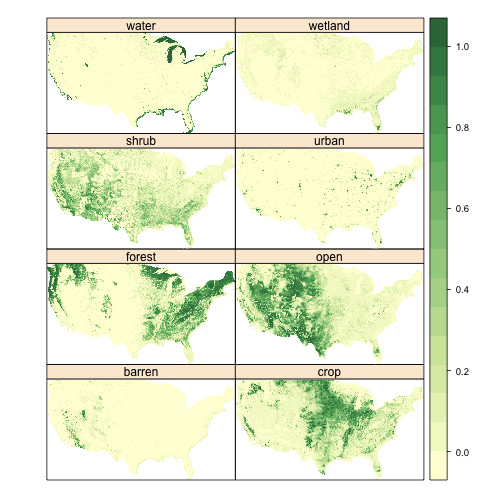
\includegraphics{fig_agc}
\caption{Final PEEL cover maps after adjusting non-crop covers to Agland2000 where possible} 
\label{fig:agc} 
\end{figure} 

\begin{figure}[ht] 
  \centering


\includegraphics{fig_agc2}
\caption{Final PEEL cover maps after adjusting non-crop covers to Agland2000 where possible (cont.)} 
\label{fig:agc2} 
\end{figure} 




% latex table generated in R 2.13.0 by xtable 1.5-6 package
% Sat Jul 16 17:12:55 2011
\begin{table}[ht]
\begin{center}
\begin{tabular}{llrr}
  \hline
agland & offset & $A_{min}$ & RMSE \\ 
  \hline
TRUE & TRUE & 0.5 & 0.017 \\ 
  FALSE & TRUE & 0.5 & 0.151 \\ 
  FALSE & FALSE & 0.5 & 0.165 \\ 
  FALSE & FALSE & 1.0 & 0.180 \\ 
   \hline
\end{tabular}
\caption{RMSE of PEEL vs. Agland2000}
\label{tab:rmse3}
\end{center}
\end{table}
% latex table generated in R 2.13.0 by xtable 1.5-6 package
% Sat Jul 16 17:13:01 2011
\begin{table}[ht]
\begin{center}
{\small
\begin{tabular}{rrrrrr}
  \hline
 & Agland2000 & NLCD & \pbox[c][][c]{3in}{MLCT\\No Mosaic} & \pbox[c][][c]{3in}{\smallskip{}MLCT\\Adjusted\\No Mosaic} & PEEL \\ 
  \noalign{\smallskip} \hline
water & 0.0 & 96.5 & 74.3 & 96.5 & 96.6 \\ 
  forest & 0.0 & 513.2 & 410.8 & 355.7 & 380.9 \\ 
  shrub & 0.0 & 420.1 & 387.2 & 358.0 & 362.8 \\ 
  open & 557.1 & 429.6 & 538.7 & 514.9 & 479.1 \\ 
  wetland & 0.0 & 95.0 & 26.0 & 95.0 & 95.0 \\ 
  crop & 446.5 & 310.8 & 495.4 & 437.6 & 443.7 \\ 
  urban & 0.0 & 102.8 & 27.3 & 102.8 & 102.8 \\ 
  mosaic & 0.0 & 0.0 & 0.0 & 0.0 & 0.0 \\ 
  barren & 0.0 & 24.5 & 32.8 & 31.9 & 31.7 \\ 
  (all) & 1003.7 & 1992.5 & 1992.5 & 1992.5 & 1992.5 \\ 
   \noalign{\smallskip} \hline
\end{tabular}
}
\caption{PEEL acreages, $A_{min}=0.5$}
\label{tab:areas3}
\end{center}
\end{table}
\todo{Discuss implications of final area tabulation}
 

\begin{figure}[ht] 
  \centering

    \includegraphics{fig_hexPlotAgc}
  \caption{Hexbin plot of PEEL crop versus Agland2000 crop}
  \label{fig:hexPlotAgc} 
\end{figure} 



\begin{sidewaysfigure}[ht] 
  \centering


    \includegraphics{fig_agcThemeMap}
  \caption{Thematic map of conflicts between NLCD offsets and Agland2000}
  \label{fig:agcThemeMap} 
\end{sidewaysfigure} 


\autoref{fig:agcThemeMap} shows a thematic map that classifies the
cells in our study area according to their agreement on the cropland
fraction between Ramankutty's Agland2000 data set and the newly
created PEEL data set.  The first class indicated by ``PEEL = 0'' in
the legend represents where Agland2000 cropland fraction is zero so
there is no potential for conflict.  The second class shows where the
PEEL crop fraction is greater than zero but Agland2000 is null,
meaning no data was given for those cells.  Such cells generally occur
in coastal areas and on the shores of the Great Lakes, reflecting that
Rmankutty's criteria for counting a cell as ``dry land'' was somehow
more restrictive.  The third class shows where the NLCD ``truth''
classes (water, wetland, urban) allowed us to bring the PEEL crop
fraction in line with Agland2000 without violating the assumption that
those fractions should be carried over from the NLCD aggregation.  The
fourth class reveals where those constraints could not be
simultaneously satisfied.  Those cells correspond to the bins in
\autoref{fig:hexPlotAgc} that fall below the equality line because the
values from the NLCD offsets are given precedence and the crop
fraction is limited accordingly, which of course might mean that other
non-offset, non-crop classes could be summarily reduced to zero.  The
final class highlights pixels that Agland2000 assigns a crop fraction
of 1.0 which seems unrealistic given that some infrastructure and
uncultivated cover must be present within such large areas.

\section{Disaggregation of PEEL Crop Fractions According to 175Crops2000}
\label{sec:peel}





\begin{figure}[ht] 
  \centering

    \includegraphics{fig_cropSubClassesMap}
  \caption{Normalized fractions for crop sub-classes}
  \label{fig:cropSubClassesMap} 
\end{figure} 

\begin{figure}[ht] 
  \centering

    \includegraphics{fig_cropSubClassesMap2}
  \caption{Normalized fractions for crop sub-classes (cont.)}
  \label{fig:cropSubClassesMap2} 
\end{figure} 


We could assume that forage crops come from open class but we don't
know enough about the confusion between Aglands2000 pasture and the
open class in the first place, much less to make an informed
speculation about how forage crops would be classified by MLCT.  The
focus here is field crops so that is the only class that we are
attempting to disaggregate and forage crops are included there for
now.  Tree and shrub crops could be taken from the corresponding cover
types, but assuming that they are caught up in that classification is
a blind leap and their areas are small.  On the other hand, their
economic impact may be disproportionate to their areas by virtue of
price, but this will have to be studied more carefully.

Double-cropping is ignored for now by normalizing the crop fractions
by the sum of all crops, which can exceed unity in instances of
intense double-cropping.  The predominant double-cropping system in
the cUSA to our knowledge is soy followed by winter wheat, but there
may be others such as multiple cropping of rice in the southern
extremes of its range.  In areas where soy and wheat are
double-cropped their areas will be underestimated in this data set
relative to that given in the 175Crops2000 data set, subsequent to the
NLCD offset adjustment.  This issues also bears further study.




%%% Local Variables: 
%%% mode: latex
%%% TeX-master: "thesis"
%%% End: 



\chapter{Conclusions}
\label{cha:conclusions}

The goal of this study was to produce a LULC data set that was as
accurate as possible with respect to its representation of the
distribution of agricultural production and that also offers a
reasonable characterization of non-crop covers and land use beyond
those agricultural uses.  We have accomplished that.  In doing so we
have adopted a sub-pixel data structure for conveying land use and
land cover information, albeit at a low spatial resolution by today's
remote sensing and GIS standards.  However, we hope that our readers
will consider that this data structure has particular mathematical
properties that may make it useful for their applications.  The
ability to perform raster algebra on these stacks of maps made it
possible to apply scaling factors and offsets with concise syntax in
the \texttt{R} language that would not have been feasible in a
discrete, categorical framework.

We maintain that the reproducible research aspect of this study was
critical to its success.  By elaborating the analysis in an
interactive environment where every component of every data structure
is subject to inspection many missteps were discovered in the course
of our work.  In other GIS analysis environments it might have been
too difficult to perform basic sanity checks on intermediate outputs
before moving on and too easy to rely on a sense of ``everything looks
right'' in a GUI environment.  The ability to point to a body of
source code that expresses the steps of the analysis is a poignant
example of reproducibility, a pillar of the scientific method that has
fallen out of vogue because of the complexity of modern spatial
analysis until the recent emergence of applicable software tools
coupled with adequate computing resources.

This analysis would not have been possible without the \texttt{raster}
package for \texttt{R} developed by Hijmans, van~Etten and other
contributors.  We consider this interface to geospatial raster data
sets in the \texttt{R} statistical analysis environment an important
contribution to spatial analysis and a laudable accomplishment because
it unleashes the power of a sophisticated, popular, open-source, free
software programming language for statistical operations on large
geospatial raster data sets.  We expect that this demonstration will
foster additional interest in and use of this software, as well as
contribution to its continuing development.  Directions for possible
enhancement that would increase the utility of this package based on
our experience include streamlining a truly functional programming
interface by improving on the existing \texttt{overlay()} function,
harnessing available \texttt{R} extensions for parallelism and porting
core functionality to a \texttt{C} or \texttt{C++} library to improve
performance, and improving the visualization interface, perhaps
through application of the \texttt{ggplot2} package as we have done
here.

In the CIM-EARTH/PEEL research agenda the next logical extension of
the envisioned land use transition model would be to apply it to a
global study area.  Once a method for creating a global initialization
data set for the year 2001 is formulated we would like to apply that
method to the subsequent years of the MLCT time series.  In order to
do so we would need ancillary data that spatially extends the aspects of the
NLCD that we have employed and temporally extends the information
given in the Ramankutty \& Monfreda data sets.  At this time a method
for calculating the correction offsets for over-estimation of cropland
and under-estimation of inland water features, wetlands, and
development/transportation infrastructure over a wider area with
greater time depth has not been identified.  Only with this
information in hand were we able bring MLCT cropland and Agland2000
cropland into close enough agreement to minimize the mathematical
manipulation necessary to reasonably quantify the non-crop cover and
use classes with the desired fidelity to the best-available rasterized
agricultural census data.

In the absence of high-resolution data on rural development, being the
low-density portion of PEEL's ``urban'' class that falls below MLCT's
detection threshold we propose that it might be possible to model the
over-estimation factor of the MLCT cropland class.  This factor would
be defined as the ratio of total area encompassed by the MLCT cropland
classification to acreage actually under cultivation and could
potentially be modeled as a function of classification confidence and
secondary class using the data described and produced here as a
training set.  The null hypothesis in the formulation of such a model
is that there is enough diversity among agricultural landscapes in our
cUSA study area to adequately characterize agricultural landscapes
around the world in this regard.  Similarly it might be possible to
directly model the ``urban'' percentage below the MLCT detection
threshold as a function of population density and agricultural
productivity, identifying said threshold in the process.  There is a
clear dependency between these offsets in agriculturally productive
regions so modeling them in conjunction somehow may be
constructive.  We expect that global offsets for the water and
wetland classes will be harder to obtain without corresponding proxy
statistics with which to formulate a model but perhaps we can expect
greater availability of spatially explicit catalogs of ecological
services and sensitive/protected areas in the near future that would
close these gaps in the available information.

\todo{Should we elaborate on this validation exercise in the conclusion or just leave it out?}

Comparison of this data to other available LULC characterizations,
particularly the Major Land Use (MLU) data and the Cropland Data Layer
(CDL) from the USDA, would provide useful validation metrics.


\backmatter

\bibliography{thesis}

%\appendix

\chapter{Appendix: Source Code}

\section*{PEEL processing library}
\lstinputlisting{code/peel.R}

\section*{Map rendering library}
\lstinputlisting{code/maps.R}

\section*{Code from Chapter 2}
\lstinputlisting{datasets.R}

\section*{Code from Chapter 3}
\lstinputlisting{analysis.R}

\end{document}